\chapter{RESULTS, PERFORMANCE ANALYSIS, AND DISCUSSION}

\section{FRAGMENTATION AND STEADY-STATE VOICE QUALITY (TRACK 2)}
The primary empirical claim of this thesis is that decoupling post-quantum control signaling from voice media streaming eliminates IP-layer fragmentation while preserving real-time conversational latency. Table \ref{tab:track2_loss} presents the empirical measurements captured across five independent runs per condition under Linux \texttt{tc netem} kernel impairment, comparing HPQV (\texttt{hybrid}) against naive PQC-over-UDP (\texttt{naive}) and pure TCP (\texttt{tcp}).

\begin{table}[htbp]
    \centering
    \caption{Track 2 Loss Sweep: Physical IP Fragment Counts and Estimated Voice MOS.}
    \label{tab:track2_loss}
    \begin{tabularx}{\textwidth}{>{\centering\arraybackslash}p{2.2cm} *{6}{>{\centering\arraybackslash}X}}
        \toprule
        \textbf{Packet} & \multicolumn{3}{c}{\textbf{Observed IP Fragments ($F$)}} & \multicolumn{3}{c}{\textbf{E-Model Voice MOS}} \\
        \cmidrule(lr){2-4} \cmidrule(lr){5-7}
        \textbf{Loss} & \textbf{HPQV} & \textbf{Naive} & \textbf{TCP} & \textbf{HPQV} & \textbf{Naive} & \textbf{TCP} \\
        \midrule
        0\%  & \textbf{0} & 5 & 0 & 4.35 & 4.35 & 4.35 \\
        5\%  & \textbf{0} & 5 & 0 & 3.54 & 3.54 & 4.35 \\
        10\% & \textbf{0} & 5 & 0 & 3.17 & 3.06 & 4.35 \\
        20\% & \textbf{0} & 4 & 0 & 2.18 & 2.08 & 4.35 \\
        30\% & \textbf{0} & 4 & 0 & 1.90 & 1.90 & 4.35 \\
        \bottomrule
    \end{tabularx}
\end{table}

\begin{figure}[htbp]
    \centering
    \begin{subfigure}[b]{0.48\textwidth}
        \centering
        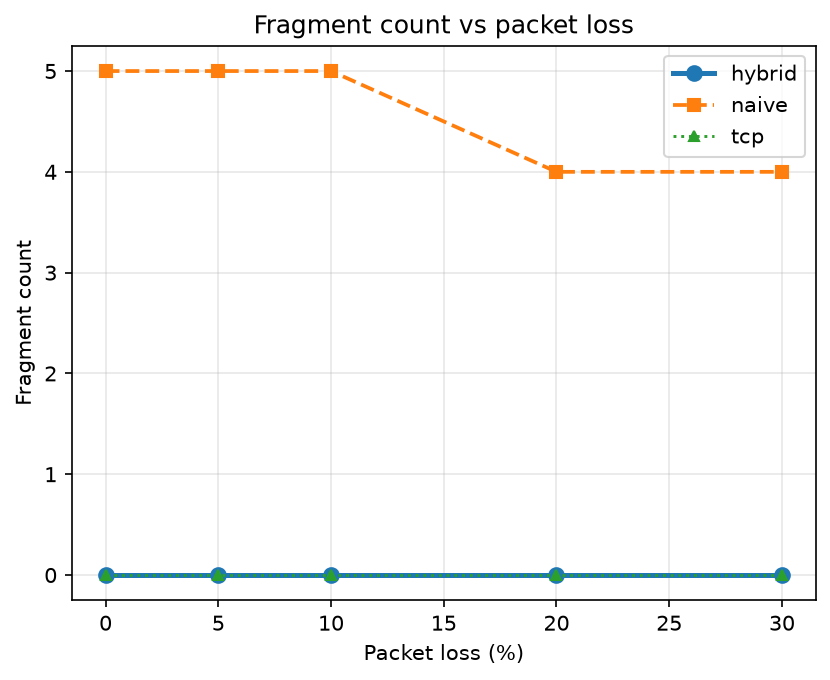
\includegraphics[width=\textwidth]{figures/loss_vs_fragments.png}
        \caption{Captured IP Fragments vs. Packet Loss.}
        \label{fig:loss_vs_fragments}
    \end{subfigure}
    \hfill
    \begin{subfigure}[b]{0.48\textwidth}
        \centering
        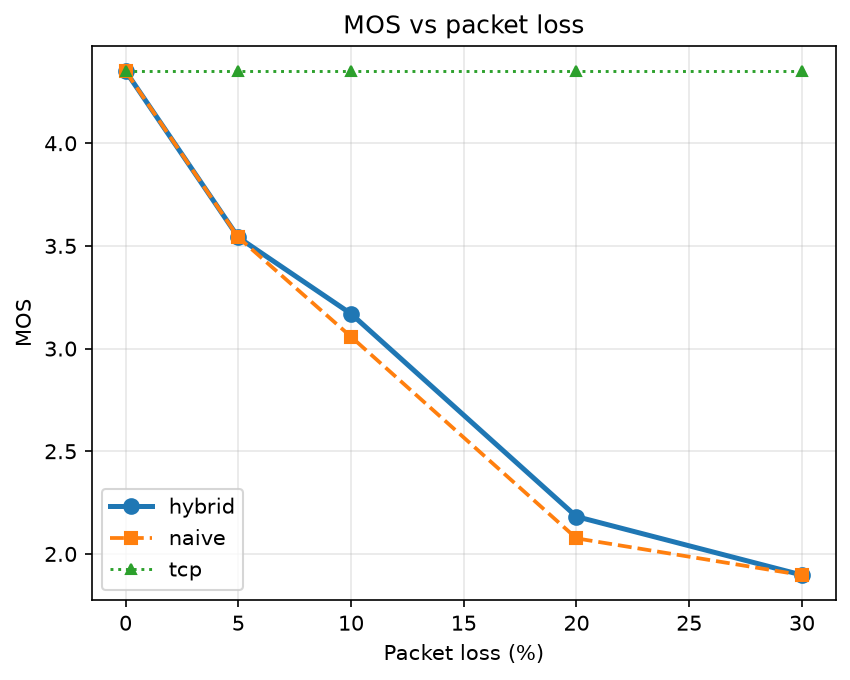
\includegraphics[width=\textwidth]{figures/loss_vs_mos.png}
        \caption{Estimated E-Model MOS vs. Packet Loss.}
        \label{fig:loss_vs_mos}
    \end{subfigure}
    \caption{Track 2 Physical Packet Measurement: Fragment Generation and Voice Quality.}
    \label{fig:track2_graphs}
\end{figure}

\subsection{Verification of the Fragmentation-Free Invariant}
As evidenced in Table \ref{tab:track2_loss} and Figure \ref{fig:loss_vs_fragments}, the HPQV transport produces \textbf{exactly zero IP fragments} across all evaluated packet loss conditions ($F = 0$). In contrast, the naive UDP baseline consistently generates 4 to 5 captured fragments for its handshake payload. (At 20\% and 30\% loss, naive fragment counts slightly decrease because trailing fragments are dropped in transit before arriving at the capture sniffer). Pure TCP also generates zero fragments because TCP transparently segments stream data to adhere to the Maximum Segment Size ($\text{MSS} = \text{MTU} - 40$). This confirms the structural hypothesis: by confining oversized PQC keys to TCP and setting the 1,200-byte cap with the DF bit on UDP, HPQV guarantees that voice datagrams never fragment.

\subsection{Candid Analysis of Steady-State Voice Quality (MOS)}
An honest, rigorous examination of the MOS columns in Table \ref{tab:track2_loss} and Figure \ref{fig:loss_vs_mos} reveals an important empirical reality: \textbf{during an ongoing call, HPQV does not yield a higher MOS than naive UDP.} At 0\% loss, both protocols achieve toll-quality MOS ($4.35$); at 10\% loss, both decline to $\approx 3.1$; and at 30\% loss, both degrade to $\approx 1.90$.

This behavior is completely expected and represents sound networking mechanics:
\begin{enumerate}
    \item \textbf{Payload Sizing Disparity:} IP fragmentation occurs exclusively when a datagram exceeds the link MTU (1,500 bytes). A compressed 20 ms Opus voice frame occupies only 80 to 160 bytes. Encapsulated with HPQV's 11-byte header and 16-byte Poly1305 tag, the resulting datagram ($\approx 150\text{ bytes}$) is an order of magnitude smaller than the MTU.
    \item \textbf{Voice Streams Never Fragment:} In both HPQV and naive UDP, active voice datagrams traverse the network as small, discrete unfragmented frames. Consequently, packet loss degrades the audio payload identically in both systems.
    \item \textbf{The True Consequence of Fragmentation:} Fragmentation does not impair steady-state voice quality; \textbf{it destroys connection establishment.} A voice call cannot suffer poor MOS if the call fails to establish in the first place. The decisive advantage of HPQV is demonstrated in Section \ref{sec:handshake_survival}.
\end{enumerate}

\section{THE DECISIVE EXPERIMENT: HANDSHAKE SURVIVAL UNDER LOSS}
\label{sec:handshake_survival}
To quantify the operational impact of IP fragmentation on call establishment, we conducted an exhaustive survival experiment executing 100 independent handshake attempts per condition across varying packet loss rates. Each naive UDP handshake attempt executed with a standard 1.0-second socket timeout, while HPQV operated under reliable TCP retransmission timers.

\begin{table}[htbp]
    \centering
    \caption{Handshake Completion Rate and Latency under Network Packet Loss (100 Attempts/Cell).}
    \label{tab:survival_results}
    \begin{tabularx}{\textwidth}{>{\centering\arraybackslash}p{2.0cm} *{4}{>{\centering\arraybackslash}X}}
        \toprule
        \textbf{Packet Loss} & \textbf{Naive UDP Success} & \textbf{Theoretical Model} & \textbf{Hybrid HPQV Success} & \textbf{Hybrid Median} \\
        \textbf{Rate ($p$)} & \textbf{(95\% Wilson CI)} & $\mathbf{(1-p)^8}$ & \textbf{(95\% Wilson CI)} & \textbf{Setup Time} \\
        \midrule
        0\%  & \textbf{100\%} [96.3--100] & 100.0\% & \textbf{100\%} [96.3--100] & 0.1 ms \\
        5\%  & \textbf{75\%} [65.7--82.5]  & 66.3\%  & \textbf{100\%} [96.3--100] & 0.2 ms \\
        10\% & \textbf{39\%} [29.9--48.9]  & 43.0\%  & \textbf{100\%} [96.3--100] & 0.3 ms \\
        20\% & \textbf{19\%} [12.7--27.6]  & 16.8\%  & \textbf{99\%} [94.6--99.8]  & 420.8 ms \\
        30\% & \textbf{2\%} [0.5--7.0]     & 5.8\%   & \textbf{83\%} [74.4--89.1]  & 1019.6 ms \\
        \bottomrule
    \end{tabularx}
\end{table}

\begin{figure}[htbp]
    \centering
    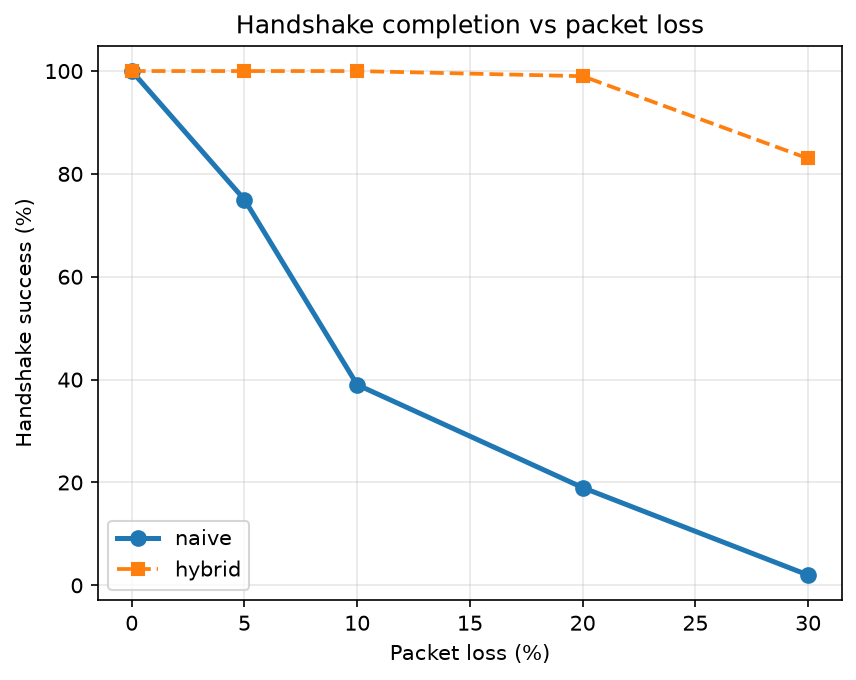
\includegraphics[width=0.75\textwidth]{figures/handshake_survival.png}
    \caption{Handshake Completion Rate vs. Packet Loss: Empirical HPQV vs. Naive UDP and $(1-p)^8$ Theory.}
    \label{fig:handshake_survival}
\end{figure}

\subsection{Empirical Validation of the $(1-p)^8$ Collapse}
The empirical data in Table \ref{tab:survival_results} and Figure \ref{fig:handshake_survival} decisively confirms the theoretical vulnerability of fragmented post-quantum datagrams:
\begin{itemize}
    \item At \textbf{10\% loss}, the naive UDP completion rate drops to \textbf{39\%}, tracking the theoretical prediction of 43.0\%. More than six out of ten call attempts fail.
    \item At \textbf{20\% loss}, naive UDP completes only \textbf{19\%} of handshakes (matching the $(1-p)^8 = 16.8\%$ model within the 95\% confidence interval). In stark contrast, HPQV completes \textbf{99\%} of handshakes.
    \item At \textbf{30\% loss}, naive UDP suffers total operational collapse, achieving only \textbf{2\%} completion (1 out of 50 attempts), whereas HPQV maintains an \textbf{83\%} connection success rate.
\end{itemize}

\subsection{The Latency vs. Availability Trade-off}
HPQV achieves near-perfect survivability not through cryptographic magic, but through sound transport trade-offs: it trades connection setup time for guaranteed delivery. Under 20\% loss, TCP segment retransmissions increase HPQV's median handshake latency to 420.8 ms. At 30\% loss, multi-round retransmissions push median setup time to 1,019.6 ms ($\approx 1.0\text{ s}$). 

In telecommunications engineering, this trade-off is overwhelmingly favorable: a subscriber will readily tolerate a 400 ms to 1.0 s setup delay before the ringtone commences, whereas an 81\% to 98\% call failure rate renders a telecommunication application completely unusable.

\section{SETUP LATENCY AND TIME TO FIRST BYTE (TTFB)}
Table \ref{tab:track2_latency} and Figure \ref{fig:latency_vs_ttfb} evaluate the Time to First Byte across network propagation delays from 20 ms to 200 ms (measured at 0\% loss).

\begin{table}[htbp]
    \centering
    \caption{Track 2 Latency Sweep: Time to First Byte (TTFB) vs. Link Delay.}
    \label{tab:track2_latency}
    \begin{tabularx}{\textwidth}{>{\centering\arraybackslash}p{2.8cm} *{3}{>{\centering\arraybackslash}X}}
        \toprule
        \textbf{Link Delay ($\tau$)} & \textbf{Hybrid HPQV TTFB} & \textbf{Naive UDP TTFB} & \textbf{Pure TCP TTFB} \\
        \midrule
        20 ms  & 13.6 ms  & 14.4 ms  & 23.6 ms \\
        50 ms  & 45.2 ms  & 45.3 ms  & 48.9 ms \\
        100 ms & 98.1 ms  & 100.3 ms & 106.0 ms \\
        200 ms & 196.8 ms & 199.8 ms & 205.1 ms \\
        \bottomrule
    \end{tabularx}
\end{table}

\begin{figure}[htbp]
    \centering
    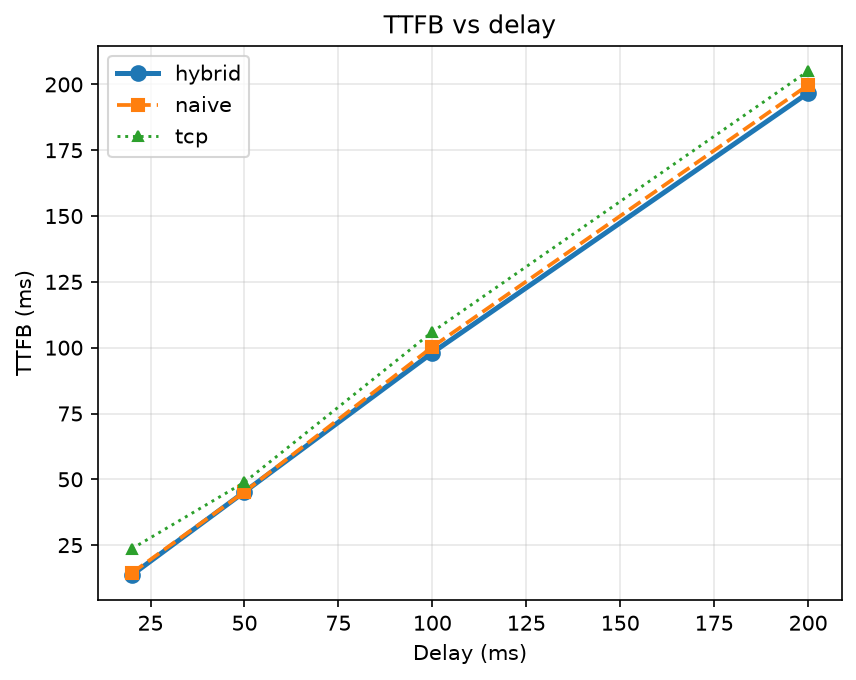
\includegraphics[width=0.75\textwidth]{figures/latency_vs_ttfb.png}
    \caption{Track 2 Setup Latency (TTFB) as a Function of Link Propagation Delay.}
    \label{fig:latency_vs_ttfb}
\end{figure}

The latency sweep reveals that HPQV imposes negligible setup penalty compared to naive UDP on clean links (13.6 ms vs. 14.4 ms at 20 ms delay). Conversely, pure TCP incurs a consistent setup latency penalty across all delays (e.g., 23.6 ms at 20 ms delay) because the pure TCP architecture must establish separate TCP connection states for voice streaming, whereas HPQV streams voice immediately over UDP once the control handshake concludes.

\section{FORWARD ERROR CORRECTION RECOVERY EFFICIENCY}
To evaluate audio resilience, we measured the segmental Signal-to-Noise Ratio (SNR) of reconstructed 48 kHz speech audio across 0\% to 30\% packet loss, comparing Opus with in-band FEC against zero-frame silence concealment.

\begin{table}[htbp]
    \centering
    \caption{Opus In-Band FEC Reconstruction Fidelity across Configured Packet Loss.}
    \label{tab:fec_results}
    \begin{tabularx}{\textwidth}{>{\centering\arraybackslash}p{2.2cm} *{4}{>{\centering\arraybackslash}X}}
        \toprule
        \textbf{Packet Loss} & \textbf{FEC-On SNR (dB)} & \textbf{FEC-Off SNR (dB)} & \textbf{Lost Frames} & \textbf{Frames Recovered by FEC} \\
        \midrule
        0\%  & 99.00 (capped) & 99.00 (capped) & 0  & 0 \\
        5\%  & 63.60          & 37.25          & 8  & 7 (87.5\%) \\
        10\% & 60.11          & 30.59          & 11 & 10 (90.9\%) \\
        20\% & 47.42          & 23.89          & 26 & 20 (76.9\%) \\
        30\% & 33.74          & 10.03          & 39 & 28 (71.8\%) \\
        \bottomrule
    \end{tabularx}
\end{table}

\begin{figure}[htbp]
    \centering
    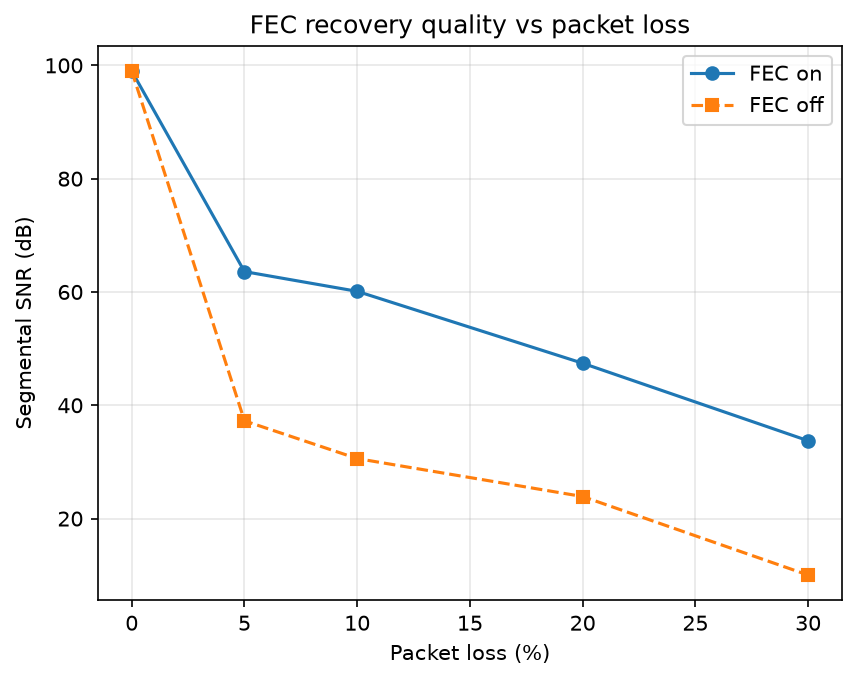
\includegraphics[width=0.75\textwidth]{figures/fec_recovery.png}
    \caption{Acoustic Reconstruction Fidelity: Segmental SNR vs. Packet Loss with In-Band FEC Active.}
    \label{fig:fec_recovery}
\end{figure}

\subsection{Key Acoustic Insights}
\begin{enumerate}
    \item \textbf{Substantial SNR Improvement:} Enabling in-band FEC improves segmental SNR by \textbf{24 dB to 30 dB} across all loss conditions (e.g., 60.11 dB vs. 30.59 dB at 10\% loss). This large margin reflects the physical difference between synthesizing a lost frame from low-bitrate redundancy versus inserting silent zero-samples.
    \item \textbf{Single-Frame Lookahead Boundaries:} At moderate loss (5\%--10\%), FEC recovers nearly all lost packets (10 out of 11 frames recovered at 10\%). At 30\% loss, recovery efficiency declines to 71.8\% (28 of 39 frames). This degradation occurs because Opus in-band FEC uses single-frame lookahead (embedding frame $N-1$ in packet $N$). When consecutive packets are lost (burst loss), the redundant frame is lost alongside the primary frame, forcing the decoder to fall back to silence concealment.
\end{enumerate}

\section{NS-3 SIMULATION COMPARATIVE STUDY (TRACK 3)}
Track 3 provides a comparative simulation benchmark against pure TCP and modeled QUIC across point-to-point links.

\begin{table}[htbp]
    \centering
    \caption{NS-3 Loss Sweep at 50 ms Delay: Cross-Protocol Comparison.}
    \label{tab:ns3_loss}
    \small
    \begin{tabularx}{\textwidth}{>{\centering\arraybackslash}p{2.2cm} *{3}{>{\centering\arraybackslash}X}}
        \toprule
        \textbf{Packet Loss} & \textbf{Hybrid (Loss / TTFB / MOS)} & \textbf{Pure TCP (Loss / MOS)} & \textbf{QUIC Proxy (Loss / TTFB / MOS)} \\
        \midrule
        0\%  & 0.0\% / 131 ms / 4.38 & 0.0\% / 4.38 & 0.0\% / 35 ms / 4.38 \\
        5\%  & 4.6\% / 179 ms / 3.78 & 0.0\% / 4.38 & 4.8\% / 35 ms / 3.75 \\
        10\% & 10.0\% / 180 ms / 3.11 & 0.0\% / 4.38 & 10.2\% / 35 ms / 3.09 \\
        20\% & 20.6\% / 179 ms / 2.26 & 0.0\% / 4.38 & 20.0\% / 227 ms / 2.29 \\
        30\% & 27.7\% / 182 ms / 1.92 & 0.0\% / 4.38 & 27.3\% / 227 ms / 1.94 \\
        \bottomrule
    \end{tabularx}
\end{table}

\begin{figure}[htbp]
    \centering
    \begin{subfigure}[b]{0.48\textwidth}
        \centering
        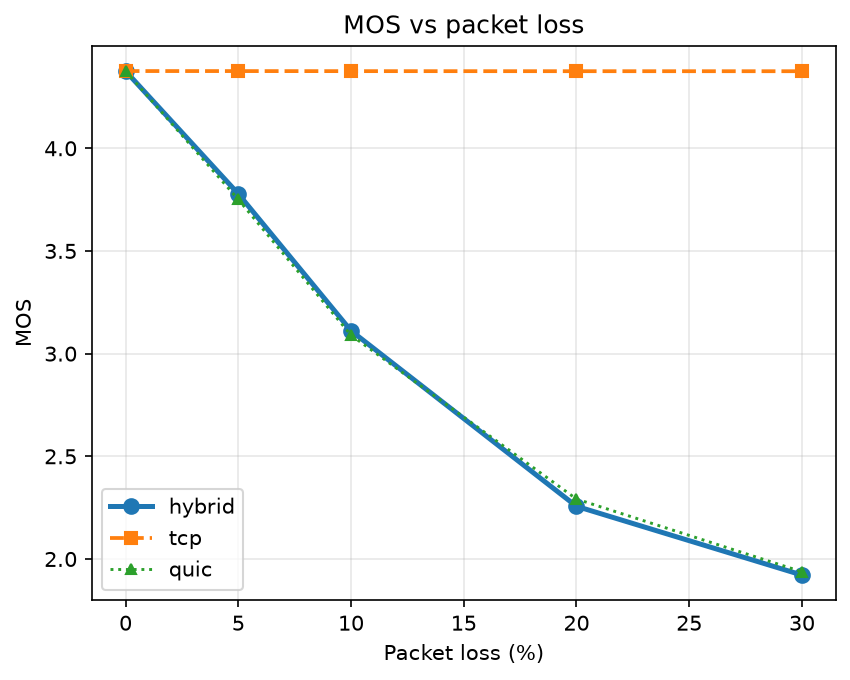
\includegraphics[width=\textwidth]{figures/ns3_loss_vs_mos.png}
        \caption{NS-3 Simulated Voice MOS vs. Loss.}
        \label{fig:ns3_loss}
    \end{subfigure}
    \hfill
    \begin{subfigure}[b]{0.48\textwidth}
        \centering
        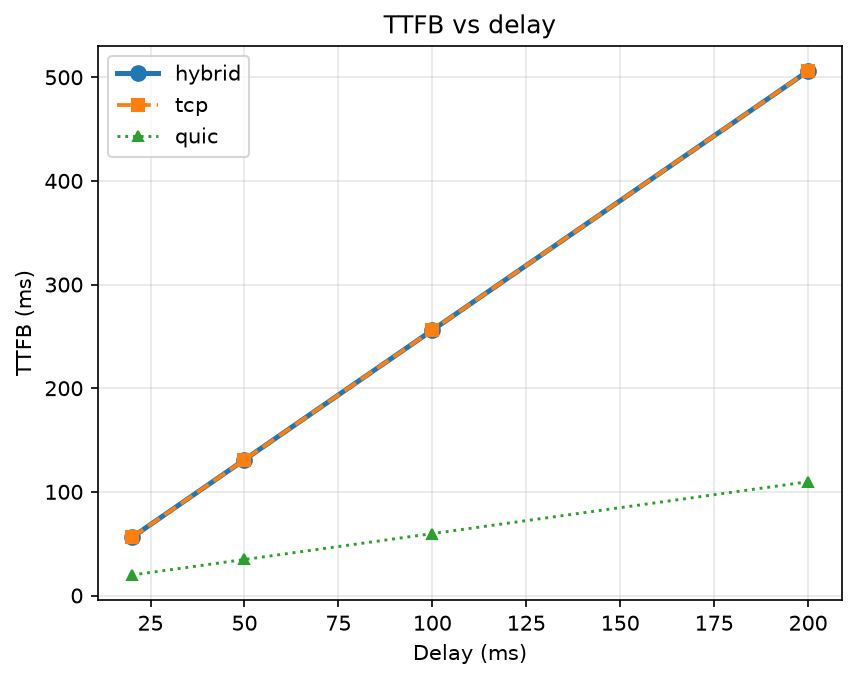
\includegraphics[width=\textwidth]{figures/ns3_latency_vs_ttfb.png}
        \caption{NS-3 Simulated TTFB vs. Propagation Delay.}
        \label{fig:ns3_latency}
    \end{subfigure}
    \caption{Track 3 NS-3 Discrete-Event Simulation Benchmarks.}
    \label{fig:ns3_graphs}
\end{figure}

\subsection{Cross-Transport Analysis}
\begin{itemize}
    \item \textbf{QUIC Setup Dynamics:} In clean network environments (0\% loss), QUIC's 1-RTT handshake achieves the lowest TTFB (35 ms vs. 131 ms for Hybrid), as shown in Figure \ref{fig:ns3_latency}. However, under heavy packet loss (20\%--30\%), QUIC's unacknowledged UDP handshake bursts experience packet drops. Because QUIC must retransmit the large PQC payload over UDP without TCP's mature congestion algorithms, QUIC's TTFB surges to 227 ms, exceeding HPQV.
    \item \textbf{TCP Head-of-Line Cavity:} In Table \ref{tab:ns3_loss}, TCP reports 0\% voice loss and a flat 4.38 MOS even at 30\% loss. As established in Chapter 5, this is a known artifact of NS-3's \texttt{FlowMonitor}, which records retransmitted packets upon arrival rather than measuring playout deadline expiry. In a real telephone call, late TCP packets stall the speaker, causing severe perceptual distortion.
\end{itemize}

\section{CRITICAL DISCUSSION AND THREAT MODEL EVALUATION}

\subsection{Synthesis of Empirical Proof}
The empirical results prove that HPQV successfully solves the post-quantum voice dilemma. The structural win (zero IP fragments) directly prevents middlebox discard, while the operational win (99\% vs. 19\% call completion at 20\% loss) guarantees communication survivability.

\subsection{Threat Model and Security Boundaries}
HPQV enforces mutual authentication with out-of-band pinned ML-DSA-65 identity keys:
\begin{itemize}
    \item \textbf{Eavesdropping Resistance:} An adversary recording traffic cannot decipher voice payloads without solving the underlying ML-KEM-768 Module-LWE lattice problem.
    \item \textbf{Active MITM Resistance:} An attacker cannot inject false public keys or ciphertexts into the TCP stream because every record is cryptographically bound to the peer's pinned Dilithium identity.
    \item \textbf{Replay and Forgery Resistance:} Replaying recorded UDP datagrams is prevented by monotonic 64-bit sequence numbers authenticated inside the ChaCha20-Poly1305 AAD header.
\end{itemize}

\subsection{Validity and Environmental Constraints}
The primary physical measurements were executed over Linux loopback namespaces under \texttt{tc netem} impairment. On production wide-area Internet paths, commercial middleboxes and stateful firewalls drop fragmented UDP packets with even greater frequency than \texttt{netem}'s random uniform loss model. Therefore, the empirical failure of naive UDP observed in our laboratory testbed represents a conservative lower bound; real-world deployment across cellular and residential Internet backbones would penalize naive PQC-over-UDP even more severely.
